\documentclass{book}
\usepackage[UTF8]{ctex}         % 使 latex支持中文
\usepackage{cite}               % 导入引用的包,能够使用\cite
\usepackage{color,xcolor}
\usepackage{multirow}           % 用于table多行合并, multicolumn已经内嵌无需导入
\usepackage{multicol}
\usepackage{ragged2e}           % 用于控制文本对齐方式
\usepackage{threeparttable}     % 用于添加tablenotes
\usepackage{float}              % 用于table, figure等的悬浮方式,[H]紧跟上一内容
\usepackage{graphicx}
\usepackage{subfigure}
\usepackage{amsmath}
\usepackage{amssymb}            % \mathbb{ctx}将内容变成花体(适用于大写字母),如期望 E,维度 R
\usepackage[lined,boxed,commentsnumbered]{algorithm2e}
                                % 算法 \begin{algorithm} ... \end{algorithm}
\usepackage{ulem}               % \uline等高下划线
\usepackage{geometry}
\geometry{left=1cm,right=1cm,top=1.5cm,bottom=1.5cm}    % 指定页边距
\usepackage{hyperref}           % [backref]表示引用表用用矩形强调, 生成书签目录
\hypersetup{hypertex=true,
            colorlinks=true,    % 是否给链接标志着色
            linkcolor=blue,     % 链接标志所着颜色
            anchorcolor=blue,
            citecolor=red}     % ref的编号颜色            

% 使图片能在分栏命令multicols中显示(使用figurehere替代figure)
\makeatletter
\newenvironment{figurehere}
    {\def\@captype{figure}}
    {}
\makeatother

\begin{document}
\title{走近NLP}
\date{}     % 空内容可除去默认添加的日期
\author{Bigluo}   % 作者
\maketitle
\flushleft  % 左对齐
\justifying % 两端对齐

\chapter{NLP团队总览}

% HuggingFace
\section{HuggingFace抱抱脸}\label{com:HuggingFace}
Hugging face 是一家总部位于纽约的聊天机器人初创服务商,开发的应用在青少年中颇受欢迎,相比于其他公司,Hugging Face更加注重产品带来的情感以及环境因素。但更令它广为人知的是Hugging Face专注于NLP技术,拥有大型的开源社区。尤其是在github上开源的自然语言处理,预训练模型库 Transformers,已被下载超过一百万次,\href{https://github.com/huggingface/transformers}{HiggingFace repo}

\begin{itemize}
    % Distill Bert
    \item 2019 Oct, \textit{Distill Bert} \cite{DistilBert}
\end{itemize}


% DeepMind
\section{DeepMind}\label{com:DeepMind}

% Google
\section{Google AI谷歌人工智能}\label{com:GoogleAI}

\begin{itemize}
    \item 2017 Jun, \textit{\hyperref[model:Transformer]{Transformer}}\cite{Transformer}
    \item 2018 Apr, \textit{Adafactor}\cite{Adafactor}
    \item 2018 Oct, \textit{Bert}\cite{Bert}
    \item 2019 Sep, \textit{Albert}\cite{Albert}
    \item 2019 Oct, \textit{\hyperref[model:T5]{T5}}\cite{T5}
    \item 2020 Jan, \textit{Reformer}\cite{Reformer}
    \item 2020 Feb, \textit{GLU-Variants}\cite{Glu-variants} 各种门控线性单元变体
    \item 2020 Feb, \textit{SimCLR}\cite{SimCLR}
    \item 2021 Aug, \textit{\hyperref[model:ST5]{Sentence T5 (ST5)}}\cite{Sentence-T5}
\end{itemize}

% FAIR
\section{FAIR facebook人工智能研究院}\label{com:FAIR}

\begin{itemize}
    \item 2019 Apr, \textit{Poly-Encoders}\cite{Poly-Encoders}
    \item 2019 Jul, \textit{Roberta}\cite{Roberta}
    \item 2019 Aug, \textit{Vilbert}\cite{Vilbert}
    \item 2019 Nov, \textit{MoCo}\cite{MoCo}
    \item 2020 Mar, \textit{MoCo-2}\cite{MoCo-2}
\end{itemize}

% OpenAI
\section{OpenAI}\label{com:OpenAI}

\begin{itemize}
    \item 2018, \textit{GPT-1}\cite{GPT-1}
    \item 2019, \textit{GPT-2}\cite{GPT-2}
    \item 2019 Apr, \textit{Sparse Transformer}\cite{Spare-Transformer}
    \item 2020 May, \textit{GPT-3}\cite{GPT-3}
    \item 2021 Feb, \textit{CLIP}\cite{CLIP}
\end{itemize}

% Microsoft Research
\section{Microsoft Research微软研究院}\label{com:MSR}

\begin{itemize}
    \item 2017 Dec, \textit{LightGBM}\cite{LightGBM}
    \item 2019 Jan, \textit{Multi-Task DNN}\cite{MT-DNN}
    \item 2019 May, \textit{UniLM}\cite{UniLM}
    
\end{itemize}

% Allen AI
\section{AllenAI}\label{com:AllenAI}

\begin{itemize}
    \item 2016 Feb, \textit{Weight Normalization}\cite{WeightNormalization}
    \item 2020 May, \textit{UnifiedQA}\cite{UnifiedQA}
    \item 2021 Mar, \textit{Unicorn}\cite{Unicorn}
    
\end{itemize}

% Tsinghua AI
\section{Tsinghua}\label{com:Tsinghua}

\begin{itemize}
    \item 2020 Dec, \textit{CPM-1}\cite{CPM-1}
    \item 2021 Jun, \textit{CPM-2}\cite{CPM-2}
    \item 2021 Mar, \textit{M6}\cite{M6}
    \item 2021 Apr, \textit{SimCSE}\cite{SimCSE}
\end{itemize}

% BAAI
\section{BAAI 北京智源人工智能研究院}\label{com:BAAI}

\begin{itemize}
    \item 2021 Jun, \textit{CPM-2}\cite{CPM-2}
\end{itemize}

% Alibaba
\section{Alibaba阿里巴巴}\label{com:Alibaba}

\begin{itemize}
    \item 2021 Mar, \textit{M6}\cite{M6}
\end{itemize}



% Baidu
\section{Baidu AIG 百度人工智能研究院}\label{com:Baidu AIG}

\begin{itemize}
    \item 2019 Apr, \textit{ERNIE-1.0}\cite{ERNIE-1.0}
    \item 2019 Jul, \textit{ERNIE-2.0}\cite{ERNIE-2.0}
    \item 2019 Oct, \textit{PLATO-1}\cite{PLATO-1}
    \item 2020 Jun, \textit{PLATO-2}\cite{PLATO-2}
    \item 2020 Jun, \textit{ERNIE-vil}\cite{ERNIE-vil}
    \item 2021 Feb, \textit{Knover}\cite{Knover}
\end{itemize}

% IFlyTek
\section{IFlyTek 科大讯飞}

\begin{itemize}
    \item 2019 Jun, \textit{Bert-wwm}\cite{Bert-wwm}
    \item 2020 Mar, \textit{Electra}\cite{Electra}
    \item 2020 Apr, \textit{MacBert}\cite{MacBert}
\end{itemize}


\chapter{基于Encoder的模型}
\chapter{基于Decoder的模型}
\chapter{基于Encoder-Decoder的模型}

% Transformer
\section{Transformer}\label{model:Transformer}

\begin{multicols}{2} 
    \begin{figurehere}
    \centering
    
    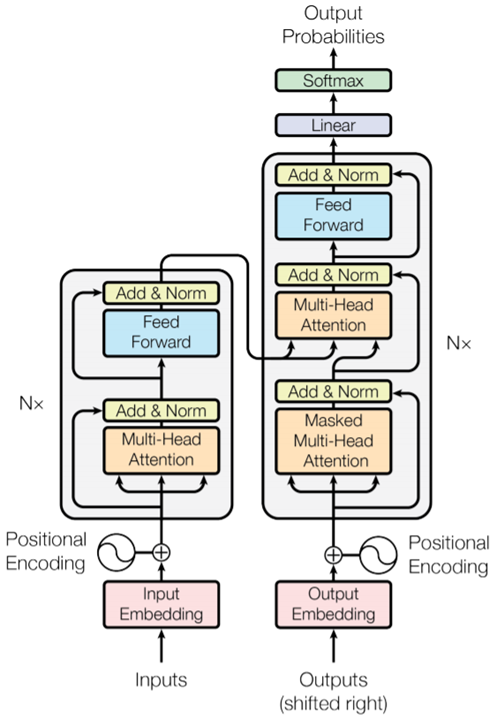
\includegraphics[width=9cm]{Encoder-Decoder/Transformer/Images/Trm Architecture.jpg}
    \caption{Transformer模型架构}
    \label{Trm:architecture}
\end{figurehere}
    %\noindent \textbf{Encoder}
    
    \begin{itemize}
        \justifying
        \item Input Embedding: 输入的token sequence embedding
        
        \item Positional Encoding位置编码满足下列特性
        1) 每个位置有唯一的位置编码
        \begin{align}
            PE(pos,2i)&=sin(\frac{pos}{1000^\frac{2i}{d_{model}}})\\
            PE(pos,2i+1)&=cos(\frac{pos}{1000^\frac{2i}{d_{model}}})
        \end{align}
        2) 由三角函数加法公式可求得相对距离$|pos_1-pos_2|$, 但\textcolor{red}{无法确定两个位置谁处于前面}
        \begin{equation}
            \begin{split}
                cos((pos_1-pos_2)*i)=cos(pos_1*i)cos(pos_2*i)\\
                +sin(pos_1*i)sin(pos_2*i)
            \end{split}
        \end{equation}
        
        \item Multi-Head Attention, 多头注意力模型
            \begin{enumerate}
                \item $Q_t=XW_Q, K_t=YW_K, V_t=ZW_V$; 一般Y, Z相同, 若X也相同则称为自注意力, <bs, seq, d>
                \item $Q_t$.reshape(bs, n, seq, d/n), $K_t$.reshape(bs, n, seq, d/n), $V_t$.reshape(bs, n, seq, d/n); n=\#heads
                \item Attention($Q_t$,$K_t$,$V_t$)=softmax($\frac{Q_tK_t^T + mask}{\sqrt{\textcolor{red}{d_k}}})V_t$; softmax用于归一化权重, 分母用于归一化协方差, mask矩阵中负无穷元素值表示masked token或pad; 
                \item Attention.reshape(bs, seq, d) 
            \end{enumerate}
        
        \item FNN前向回馈网络: $activate(xW_1+b_1)W_2+b_2$
        \begin{itemize}
            \item [$\triangleright$] $W_1$, $<d, d_{ff}>$
            \item [$\triangleright$] $W_2$, $<d_{ff}, d>$
        \end{itemize}
         
        \item Output Embedding: 同语种时与Input Embedding一致, 不同语种时(如处理翻译任务)则是另一Learnable Embedding
    \end{itemize}
    %\noindent Decoder
    %\begin{itemize}
    %    \item ss
    %\end{itemize}
\end{multicols}


% T5
\newpage
\section{T5}\label{model:T5}

% ST5
\section{Sentence T5 (ST5)}\label{model:ST5}
\chapter{对比学习}
\chapter{多模态}
\chapter{提升技巧}
\chapter{Optimizer优化器}
\chapter{集成学习}

\bibliography{refs}             % 需创建refs.bib文件才可生效
\bibliographystyle{ieeetr}      % 指定ref风格
\end{document}